
\section{Hybrid Function Merging} \label{sec:contribution}

In this section, we propose {\ProjName} (Hybrid Function Merging), a novel function merging technique that can operate on all functions regardless of their size with little to no compilation overheads.
%and introduces little to no end-to-end overhead, while still delivering similar or better code size reduction as the state-of-the-art.
To achieve this goal, we rely on the insights discussed in Section~\ref{sec:motivation}.
Our solution is three-fold:
1) We introduce an alignment strategy that works on the level of basic blocks, without crossing their boundaries, leading to faster and less memory demanding alignment;
2) We incorporate a multi-tier profitability analysis that allows us to bail out from unprofitable merging attempts even before code generation;
3) We introduce a linear pairwise alignment for basic blocks of the same size that produces good results on highly similar blocks.
This technique can be enabled as an alternative to the quadratic sequence alignment algorithm.
Both techniques have their place, offering different trade-offs.
%\fixme{MC: Saying "propose" here sounds a bit passive compared to the previous two points. Better to say "introduce" then make it clear that it is a complementary technique to NM, and both may have their place}

\subsection{Overview}

For all candidate functions and basic blocks, we generate a fixed-vector representation, namely, their fingerprint~\cite{rocha19,rocha20}.
We match each function with its most similar available function, the one with the shortest fingerprint distance.
Instead of aligning their linearized representations directly, we work at the basic block level.
We pair similar basic blocks of the two functions based on their fingerprint distances.
%Unlike prior work, we require no linearization of the input functions.
We align the instructions in these paired basic blocks using either the {\NW} alignment~\cite{needleman70} or our linear pairwise alignment strategy.
We employ the first-tier profitability analysis on each alignment. If the cost model deems it unprofitable, we skip the pair.
The pairing of basic blocks, the alignment, and the first-tier profitability analysis are executed in rounds, in a greedy manner.
That is, the first profitable pairing is taken, however, unprofitable paired blocks are freed for another pairing, if necessary.
%\fixme{PP: We should mention this in 3.2, 3.3, or 3.4 too. Also how does that work when we have no first-tier profitability analysis? Do we always keep the first pair or do we keep merging the functions and doing the second tier analysis for every single basic block pair we try?}

Once all basic blocks have been processed, we combine the block alignments into a function-wide one and we produce the merged function using the same code generation proposed for {\SOAName}~\cite{rocha20}.
If no profitable pair of basic blocks was found, we bail out before code generation.
Finally, we perform the second-tier profitability analysis, which is the same used by {\SOAName}, to decide whether replacing the original functions by the merged one reduces code size. If not, we reject the merged function and we keep the original ones.

For brevity, the rest of the discussion will focus on how {\ProjName} differs from previous approaches. 

%For its greedy strategy, {\ProjName} introduces the following restrictions:
%1) Instruction matching is performed only within a pair of basic blocks, without crossing their boundaries.
%2) The basic blocks paired for matching must have the same number of instructions.
%3) The match making is performed in a pairwise manner.
%We can derive a greedy alignment strategy directly from these restrictions.

%The first two restrictions can be leveraged to narrow down the search space.
%Unlike prior techniques, {\ProjName} is able to pair any two basic blocks, regardless of their position in the control-flow graph.
%Therefore, it uses a fingerprint-based technique in a similar manner to how fingerprints are used to pair functions for merging (see Section~\ref{related:salssa}).

%\subsection{Search Strategy for Pairing Functions}
%{\ProjName} uses the same search strategy as {\SOAName} to pair similar functions for merging.

%SalSSA~\cite{rocha20} has a search strategy for pairing similar functions for merging but avoiding a prohibitively expensive quadratic number of merging attempts.
%The purpose of the search strategy is to avoid a quadratic exploration that attempts to merge all possible pairs of functions.
%All three techniques use a ranking strategy based on the \textit{fingerprint} of the functions to evaluate their similarity.
%They start by precomputing and caching fingerprints for all functions.
%The fingerprint is a fixed-size vector that summarizes the content of the function.
%To this end, the fingerprint consists of a map of instruction opcodes to their frequency in the function.
%While functions can have several thousands of instructions, an IR usually has just a few tens of opcodes, e.g., the LLVM IR has only about 68 different opcodes.

%The fingerprint representation allows us to compare functions using a simple distance metric, such as the Manhattan distance.
%For a given reference function, all other functions are ranked based on the distance of their fingerprints.
%The candidate function with the smallest distance will be used for a merging attempt.


\subsection{Pairing Similar Basic Blocks}
\label{sec:bb-rank}

We pair similar basic blocks based on distance of their fingerprints.
%Figure~\ref{fig:hyfm-bb-pairing} illustrates the fingerprint-based process used to pair basic blocks.
This pairing process is similar to the search strategy used for pairing functions~\cite{rocha19}.
We use the same fingerprint, a fixed-size vector of integers with the frequency count of each opcode.
%, with well-known distance metrics.
It can be used to represent any piece of code, from basic blocks to whole functions.

The overall idea is that for each block in one function we select a block from the other function that minimizes the Manhattan distance between their fingerprints.
Formally, given a block $B_1 \in F_1$, where $F_1$ is the set of all blocks from function one, $B_1$ is paired with a block $B_m \in F_2$ such that:
\[  d(B_1,B_m) = min\{d(B_1,B_2) : B_2 \in F_2\} \]
where $d(B_1,B_2)$ represents the distance between the fingerprints of the basic blocks $B_1$ and $B_2$.

% First, for one of the input functions, we group all its blocks by their number of instructions, excluding phi-nodes.
% Then, {\ProjName} iterates over all blocks from the second input function, in no particular order, looking for a suitable candidate from the group of blocks with the same size.
% The best candidate is the basic block for which their fingerprint has the smallest distance.
% Since the fingerprint is a fixed-size vector, several well-known distance metrics can be used, such as the Manhattan distance, the cosine distance, etc.
% In this paper, we are using the Manhattan distance.

% \begin{figure}[h]
% \centering
% \includegraphics[width=0.9\linewidth]{figs/fingerprint-example.pdf}
% \vspace{-2ex}
% \caption{Example of a fingerprint.
% It is a fixed-size vector of integers with the frequency of each opcode. }
%  \label{fig:fingerprint-example}
% \end{figure}

% Formally, the hash structure can be defined as:
% \[  H[s] = \{ B_1 \in F_1 : |B_1| = s \} \]
% where $F_1$ contains the set of all basic blocks from the first input function and $|B|$ denotes the size of a given basic block.
% Therefore, a given $B_2 \in F_2$ is paired with $B_m \in H[|B_2|]$ such that:
% % %\[  B_m \in H[|B_2|] \land d(B_m,B_2) = min\{d(B_1,B_2) : B_1 \in H[|B_2|\} \]
% \[  d(B_m,B_2) = min\{d(B_1,B_2) : B_1 \in H[|B_2|\} \]
% where $d(B_1,B_2)$ represents the distance between the fingerprints of the basic blocks $B_1$ and $B_2$.


%Since the fingerprint of basic blocks have fixed size, i.e., the number of instruction opcodes, the distance between two basic blocks can be computed in constant time.


%as well as inspired by the more restrictive technique proposed by von Koch~et~al.~\cite{edler14}.


%These suitable candidate blocks are identified using a search strategy similar to the one used when searching for function candidates.
%For a given basic block $B_{2,j}$ from Function 2, 
%Basic blocks are paired by minimizing the Manhattan distance between their fingerprints, in a greedy manner.
%\[
%  \operatorname*{argmin}_{B_2 \in F_2} \{ d_1(F(B_1), F(B_2)) \} 
%\]

% \begin{figure}[h]
% \centering
% \includegraphics[width=0.8\linewidth]{figs/hyfm-ranking-full.pdf}
% \caption{Example illustrating one block from Function 2 being compared to all available blocks from Function 1. The pair with the smallest fingerprint distance will be considered for alignment.\fixme{PP: Not particularly informative imo.}}
%  \label{fig:hyfm-bb-pairing}
% \end{figure}

After pairing two basic blocks, $B_1$ and $B_2$, they have their instructions aligned (see Section~\ref{sec:bb-alignment}) and their merging profitability estimated (see Section~\ref{sec:multi-profitability}).
If they are deemed profitable, both blocks are removed from their respective working list.
Otherwise, only $B_1$ is removed from the working list of blocks from $F_1$, i.e., $B_2$ can still be paired with another block, but not $B_1$.
In other words, basic blocks from function $F_1$ are paired only once, even if its alignment is deemed unprofitable.
As a result, given two input functions, this pairing process is quadratic on their number of basic blocks.
This number is usually much smaller than the number of instructions in the function, so the cost of pairing is much lower than the cost of aligning whole functions in {\SOAName}, despite both being quadratic. For very large numbers of basic blocks, efficient nearest neighbor search techniques could keep the cost low but this was not needed in our experiments.

{\ProjName} pre-computes the fingerprint of every basic block in the input functions, which is a single linear cost over all their basic blocks and instructions.
Meanwhile, the distance between two fingerprints is computed in constant time, since the number of opcodes is a small constant.


% Note that the construction of the hash data structure is linear on the size of the functions $O(N)$ while the pairing itself can be quadratic on the number of basic blocks, $O(B^2)$.
% In the worst case, all basic blocks would have the same size and this exploration would be quadratic on the number of basic blocks.
% However, the number of basic blocks tend to be much smaller than the number of instructions and for large functions, basic blocks tend to vary in size.
% Therefore, it is unlikely that {\ProjName} will experience the worst case scenario for large functions.
% \textbf{TODO:} What is the average size of basic blocks per function (compare it with the average number of functions)? For functions with more than one basic block, how many of them have all basic blocks of the same size?

%%Given two functions, our goal is to produce a 


%To avoid breaking the semantics of the original program, we also need to maintain the order of the instructions for each of the functions.


%First, for one of the input functions, we group all its blocks by their number of instructions, except for the phi-nodes.
%We also pre-compute a fingerprint-based encoding of the basic blocks.
%This data structure allows us to quickly search for matching candidate blocks since they would have identical encodings.


%RestrictiveFM iterates over all blocks from the second input function, looking for a fully matching candidate block from the first function.

\subsection{Aligning Paired Basic Blocks}
\label{sec:bb-alignment}


%\subsubsection{\NW Alignment}
\label{sec:nw-alignment}

Basic blocks already represent a linearized sequence of instructions.
Any sequence alignment algorithm can be used on them the same way they can be used on linearized functions. The globally optimal \NW~\cite{needleman70} used by {\SOAName} remains a good choice. It may be quadratic in both space and time on the length of the sequences but basic block sequences are usually much shorter than functions, making the cost of alignment lower than in previous approaches. 

%\subsubsection{Linear Pairwise Alignment}
\label{sec:pa-alignment}

Our observations in Section~\ref{sec:motivation}, though, indicate that a globally optimal algorithm might be an excessive solution. %overkill.
Profitable sequences tend to be highly similar, so aligning them is usually straightforward. Based on this insight, we implemented a linear alignment algorithm. Its assumption is that profitable pairs of blocks are almost identical in terms of opcodes differing only in a few individual cases. This translates into a pairwise alignment of same size basic blocks where only corresponding instructions in the two blocks can match. Figure~\ref{fig:hyfm-alignment} illustrates two examples of basic blocks aligned using our strategy.
It also includes the costs estimated by our profitability analysis, which we discuss in Section~\ref{sec:multi-profitability}.

%As an alternative to the quadratic alignment algorithm, we also propose a linear alignment solution.
%This solution restricts pairing only between basic block of the same size.
%This restriction allows for a pairwise alignment, where only corresponding instructions in the paired basic blocks can match.
%Figure~\ref{fig:hyfm-alignment} illustrates two examples of basic blocks aligned using our linear pairwise strategy.

\begin{figure}[h]
\centering
  \begin{subfigure}{\linewidth}
  \center
  \includegraphics[width=0.6\linewidth]{src/lctes21/figs/hyfm-alignment-good.pdf}
  \caption{A profitable alignment. Both $OriginalCost$ and $MergedCost$ are 10. The final score is $OriginalCost - MergedCost = 0$.}
  \label{fig:hyfm-alignment-good}
  \end{subfigure}
\\
  \begin{subfigure}{\linewidth}
  \center
  \includegraphics[width=0.6\linewidth]{src/lctes21/figs/hyfm-alignment-bad.pdf}
  \caption{An unprofitable alignment. $OriginalCost$ is 0 and $MergedCost$ is 15. The final score is $-3$. A negative score means it is unprofitable.}
  \label{fig:hyfm-alignment-bad}
  \end{subfigure}
\vspace{-2ex}
\caption{Two examples of the pairwise alignment. Only instructions in corresponding positions are aligned. Instructions match if they have the same opcode.}
 \label{fig:hyfm-alignment}
\end{figure}

Restricting alignment to basic blocks of the same size has the added benefit that it simplifies the pairing strategy. We only have to consider fingerprints for basic blocks of the same size, so we group them by block size and we restrict our search in the right group.
In the worst case, all basic blocks would have the same size and the search would remain quadratic on the number of basic blocks, as discussed in Section~\ref{sec:bb-rank}.
However, this is unlikely to happen in large functions, which is where the number of basic blocks might be a problem.
Overall, this solution is lean on memory usage and usually the fastest for aligning paired basic blocks, as corroborated by our evaluation in 
Section~\ref{sec:evaluation}.

\subsection{Multi-Tier Profitability Analysis}
\label{sec:multi-profitability}

{\ProjName} incorporates a multi-tier profitability analysis that enables it to bail out early from an unprofitable merge operation.
The first tier consists of a simple analysis applied on each pair of basic blocks selected for alignment, either accepting or rejecting the alignment between two blocks. 
The second tier consists of the same profitability analysis that is also performed by FMSA and {\SOAName}, which is responsible for evaluating whether the merged function is smaller than the original input functions.

The last column of Figure~\ref{fig:hyfm-alignment} shows how the first tier analysis is employed alongside the pairwise alignment strategy.
The same analysis can also be applied on pairs of basic blocks aligned using the \NW algorithm.
The analysis tries to estimate the cost of merging, the total number of instructions that will be necessary for merging the aligned blocks.
If two instructions match, then a single instruction is needed (i.e., a cost of \texttt{+1} is assigned to this entry).
If they mismatch, then both instructions are needed (i.e., a cost of \texttt{+2} is assigned to this entry).
Moreover, we need extra instructions to transition from matching subsequences to mismatching ones, and vice versa.
This is represented by the arrows in Figure~\ref{fig:hyfm-alignment}.
One branch instruction is needed to split control flow into two mismatching instructions, while two branch instructions are needed to join it back into a matching pair of instructions. 
The $MergedCost$ is the sum of all these costs.
The profitability score is defined as $OriginalCost - MergedCost$, where $OriginalCost$ is simply the number of instructions in the original basic blocks.
Therefore, a negative profitability score means that merging those two basic blocks is unprofitable. When this is the case, we ignore the alignment.

By rejecting individual basic block alignments, we are able to decide early whether merging a pair of functions might be profitable. If we rejected all block alignments, then by definition there is no point in merging the functions. Previous approaches, without a first tier analysis, have to rely on the second tier exclusively which is applied after the functions are merged.

\subsection{Independence from Code Layout}
%\fixme{MC: Is Code Reordering the right title here? As I understand it, this strength is basically because of the "consider all other blocks" aspect of the algorithm, so their source ordering becomes irrelevant. The insight is that we have decoupled the blocks from their position in the control flow. "Code Reordering" sounds like some more proactive smartness considering possible reordering, and a reader may expect to see this?  Maybe something like "Independence from Code Ordering" or some other phrase which captures this?}
Unlike all prior techniques, {\ProjName} is able to merge similar basic blocks regardless of their position in the control-flow graphs from the input functions.
Figure~\ref{fig:reordering-example} shows an example of  two functions that all prior techniques fail to merge even though they are highly similar. 

\begin{figure}[h]
  \centering
  \includegraphics[width=0.95\linewidth]{src/lctes21/figs/soplex-example-one-column.pdf}
  \caption{Example with code reordering extracted from the \texttt{450.soplex} program.}
  \label{fig:reordering-example}
\end{figure}

% \begin{figure*}[t]
%   \centering
%   \includegraphics[width=0.75\textwidth]{figs/soplex-example.pdf}
%   \caption{Example with code reordering extracted from the \texttt{450.soplex} program.}
%   \label{fig:reordering-example}
% \end{figure*}

Due to their rigid linearization strategy, both FMSA and {\SOAName} are unable to properly match the basic blocks of the if-else structure, resulting in sub-optimal merged functions that are deemed unprofitable.
Their linearization traverses the control-flow graph in a canonical manner, preventing blocks from being rearranged for a better merging~\cite{rocha19,rocha20}.
Meanwhile, earlier techniques fail to merge this example as they are restricted to functions with identical control-flow graphs where corresponding blocks are merged~\cite{livska14,edler14,llvm-fm}.

{\ProjName} is able to correctly pair these basic blocks.
Because the basic blocks are rearranged, the label operands of the conditional branch need to be handled in order to preserve the program semantics.
For swapped label operands, {\ProjName} simply uses the optimized operand resolution proposed by {\SOAName}, where an \texttt{xor} operation is applied on the condition of the branch and the function identifier~\cite{rocha20}.


